\vspace{-1mm}
\section{Experiments}
\label{sec:exp}

\vspace{-1mm}
\subsection{Experimental Setup}
\label{sec:setup}
\vspace{-1mm}

\paragraph{Backbone and benchmarks.}
We evaluate LoTR on 3 LLM backbones: \textbf{Llama-3.1-8B} \citep{grattafiori2024llama3}, \textbf{Qwen2.5-14B} \citep{yang2024qwen25}, and \textbf{Mixtral-8x7B} \citep{jiang2024mixtral} with 8 standard reasoning benchmarks spanning mathematical, scientific, logical, factual, coding, and long-form QA, including \textbf{GSM8K} \citep{cobbe2021gsm8k}, \textbf{MATH} \citep{hendrycks2021math}, \textbf{BoolQ} \citep{clark2019boolq}, \textbf{HumanEval} \citep{chen2021evaluating}, \textbf{MMLU} \citep{hendrycks2021mathmassive}, \textbf{FOLIO} \citep{han2022folio}, \textbf{HotpotQA} \citep{yang2018hotpotqa}, and \textbf{NarrativeQA} \citep{kocisky2018narrativeqa}. 

\vspace{-1mm}
\paragraph{External reasoning paradigms.}
We instantiate LoTR on Vanilla and 7 representative reasoning paradigms: 
\textbf{Chain-of-Thought} (CoT) \citep{wei2022chain}, 
\textbf{Plan-and-Solve} (PS) \citep{wang2023plan}, 
\textbf{Self-Refine} (SR) \citep{madaan2023selfrefine}, 
\textbf{Self-Consistency} (SC) \citep{wang2023selfconsistency}, 
\textbf{Best-of-$N$} (BoN) \citep{chow2024inferenceaware,lightman2024verify}, 
\textbf{Constrained Beam} (CB) \citep{hokamp2017lexically,post2018fast}, and 
\textbf{Monte Carlo Tree Search} (MCTS) \citep{xie2024mcts}. 
These paradigms span direct generation, single-path decomposition, plan-then-execute prompting, iterative revision, sample-and-aggregate scaling, sample-and-rerank scaling, constrained multi-hypothesis decoding, and explicit tree search, broadly testing whether LoTR generalizes across heterogeneous trajectories rather than overfitting to one reasoning scaffold.

\vspace{-1mm}
\paragraph{Plug-in baselines.}
Since LoTR is a frozen-backbone, inference-time, plug-in controller, the most relevant comparisons are published intervention methods that also modify internal computation without updating model weights. 
We compare against \textbf{ITI} \citep{li2023inference}, which intervenes on a selected subset of attention heads at inference time; 
\textbf{ActAdd} \citep{turner2024actadd}, which steers generation through activation addition; 
\textbf{STIR} \citep{shi2026stir}, which uses retrieved latent steering impulses to guide reasoning trajectories; and 
\textbf{RISER} \citep{ye2026riser}, which adaptively composes reusable reasoning steering signals through a router. 

\vspace{-1mm}
\paragraph{Metrics.}
Accuracy is measured by Exact Match for GSM8K, MATH, BoolQ, MMLU, FOLIO, and NarrativeQA, by F1 score for HotpotQA, and by Pass@1 for HumanEval. 
We also report generated tokens and end-to-end latency to compare the efficiency of different methods in H200.

\vspace{-1mm}
\subsection{Main Results}
\label{sec:main}
\vspace{-1mm}
\paragraph{Overall effectiveness.}
Table~\ref{tab:main_llama} reports Llama-3.1-8B accuracy across eight paradigms: LoTR leads the eight-benchmark average seven times and strictly raises every paradigm composite above its unsteered baseline.
Representative stresses echo logic-conditioned routing: Vanilla mean accuracy reaches $48.3$\% with HotpotQA at $7.6$\% while competing steers drive it near zero; Plan-and-Solve hits $32.8$\% average while preserving HumanEval at $24$\% as ITI crashes to $11.4$\%; constrained beam and Self-Consistency/Best-of-$N$ composites peak at $45.3$\%, $41.2$\%, and $40.2$\%, respectively---together arguing that outer scaffolds pay off only when interior pathways track their induced logic rather than applying a fixed impulse.
What these blocks jointly indicate---without redesigning the wrappers themselves---is LoTR's central thesis: the bottleneck under frozen weights is often mismatch between a prescribed external procedure and a still-static internal execution pathway, and coupling pathway selection to inferred logic states is what lets diverse strategies be realized more faithfully step by step.
We further provide a theoretical account of this design in Appendix ~\ref{app:theory_frontier} to \ref{app:theory_generalize}.

\vspace{-1mm}
\paragraph{Generalization.}
ITI, ActAdd, STIR, and RISER cover masking, global addition, retrieval, and routed mixtures, yet Table~\ref{tab:main_llama} shows they largely remain \emph{logic-agnostic}: Vanilla composites lag LoTR ($47.6$\%, $45.6$\%, $45.0$\%, $46.5$\% vs.\ $48.3$\%), HotpotQA collapses under ITI ($0.2$\%) while LoTR holds $7.6$\%, ActAdd even dips below no-steer ($45.6$\%/$45.8$\%), structured decoding favors LoTR ($45.3$\% vs.\ STIR $43.3$\%), decomposition widens the CoT gap to RISER ($43.8$\% vs.\ $41.3$\%), and PS exposes brittle coding when masking ignores step logic (HumanEval $11.4$\% vs.\ LoTR $24$\%).
LoTR closes this pattern by swapping cached head templates with probe-estimated state occupancy, so improvements carry across paradigms instead of trading shortcut spikes on a few axes for portfolio-wide reliability.
Mechanistically, that closure distinguishes \emph{logic-indexed} pathway control from stronger-but-blind impulses: the steer families above largely reuse interventions irrespective of which recurring logic configuration is active at the current sentence, whereas LoTR conditions interior rewiring on that configuration---which is why composites rise even when individual benchmarks disagree.
Appendix~\ref{app:pipeline_effect} further dissects this mechanism step-wise.

\begin{table*}[t]
\centering
\caption{\textbf{Main results on Llama-3.1-8B (accuracy, \%),} with other models in Table~\ref{tab:app_main_qwen}, ~\ref{tab:app_main_mixtral}}
\label{tab:main_llama}
% muted delta colors (Table~\ref{tab:main_llama})
\definecolor{lotrgain}{RGB}{178,72,72}
\definecolor{lotrloss}{RGB}{52,128,88}
% +\textbf{LoTR} accuracies: \texttt{lotr\_bingrid\_20260427T191904Z\_ll\_p3k5/k05} (best mean among evaluated \texttt{\_ll\_p\{2,3\}k\{5,6\}} bingrid runs on this snapshot). Details: \texttt{paper/data/main\_llama\_lotr\_snapshot.json}.
\vspace{-2mm}
\footnotesize
\setlength{\tabcolsep}{3pt}
\renewcommand{\arraystretch}{0.86}

\resizebox{\textwidth}{!}{%
\begin{tabular}{lccccccccc}
\toprule
\textbf{Method} & \textbf{GSM8K} & \textbf{MATH} & \textbf{BoolQ} & \textbf{HumanEval} & \textbf{MMLU} & \textbf{FOLIO} & \textbf{HotpotQA} & \textbf{NarrativeQA} & \cellcolor{gray!15}{\textbf{Average}} \\
\midrule
    Vanilla & 78.9 & 54.1 & 74.7 & 62.0 & 40.9 & 29.1 & 7.1 & 19.8 & \cellcolor{gray!15}{45.8} \\
    + ITI & 80.6\,{\textcolor{lotrgain}{\scriptsize (+1.7\%)}} & \underline{57.9}\,{\textcolor{lotrgain}{\scriptsize (+3.8\%)}} & 81.9\,{\textcolor{lotrgain}{\scriptsize (+7.2\%)}} & \underline{63.0}\,{\textcolor{lotrgain}{\scriptsize (+1.0\%)}} & 44.7\,{\textcolor{lotrgain}{\scriptsize (+3.8\%)}} & \underline{32.9}\,{\textcolor{lotrgain}{\scriptsize (+3.8\%)}} & 0.2\,{\textcolor{lotrloss}{\scriptsize (-6.9\%)}} & 19.3\,{\textcolor{lotrloss}{\scriptsize (-0.5\%)}} & \cellcolor{gray!15}{47.6\,{\textcolor{lotrgain}{\scriptsize (+1.8\%)}}} \\
    + ActAdd & 81.7\,{\textcolor{lotrgain}{\scriptsize (+2.8\%)}} & \underline{57.9}\,{\textcolor{lotrgain}{\scriptsize (+3.8\%)}} & 81.9\,{\textcolor{lotrgain}{\scriptsize (+7.2\%)}} & 61.3\,{\textcolor{lotrloss}{\scriptsize (-0.7\%)}} & 45.1\,{\textcolor{lotrgain}{\scriptsize (+4.2\%)}} & 30.3\,{\textcolor{lotrgain}{\scriptsize (+1.2\%)}} & 0.1\,{\textcolor{lotrloss}{\scriptsize (-7.0\%)}} & 6.4\,{\textcolor{lotrloss}{\scriptsize (-13.4\%)}} & \cellcolor{gray!15}{45.6\,{\textcolor{lotrloss}{\scriptsize (-0.2\%)}}} \\
    + STIR & 81.4\,{\textcolor{lotrgain}{\scriptsize (+2.5\%)}} & 56.2\,{\textcolor{lotrgain}{\scriptsize (+2.1\%)}} & 81.6\,{\textcolor{lotrgain}{\scriptsize (+6.9\%)}} & 61.2\,{\textcolor{lotrloss}{\scriptsize (-0.8\%)}} & 44.6\,{\textcolor{lotrgain}{\scriptsize (+3.7\%)}} & 29.3\,{\textcolor{lotrgain}{\scriptsize (+0.2\%)}} & 0.0\,{\textcolor{lotrloss}{\scriptsize (-7.1\%)}} & 5.5\,{\textcolor{lotrloss}{\scriptsize (-14.3\%)}} & \cellcolor{gray!15}{45.0\,{\textcolor{lotrloss}{\scriptsize (-0.8\%)}}} \\
    + RISER & 81.0\,{\textcolor{lotrgain}{\scriptsize (+2.1\%)}} & 56.2\,{\textcolor{lotrgain}{\scriptsize (+2.1\%)}} & 81.3\,{\textcolor{lotrgain}{\scriptsize (+6.6\%)}} & 61.0\,{\textcolor{lotrloss}{\scriptsize (-1.0\%)}} & 44.5\,{\textcolor{lotrgain}{\scriptsize (+3.6\%)}} & 29.1\,{\textcolor{gray!55!black}{\scriptsize (+0.0\%)}} & 0.0\,{\textcolor{lotrloss}{\scriptsize (-7.1\%)}} & 19.2\,{\textcolor{lotrloss}{\scriptsize (-0.6\%)}} & \cellcolor{gray!15}{46.5\,{\textcolor{lotrgain}{\scriptsize (+0.7\%)}}} \\
    + \textbf{LoTR} & \cellcolor{cyan!10}{\textbf{\underline{82.0}}\,{\textcolor{lotrgain}{\scriptsize (+3.1\%)}}} & \cellcolor{cyan!10}{\textbf{57.0}\,{\textcolor{lotrgain}{\scriptsize (+2.9\%)}}} & \cellcolor{cyan!10}{\textbf{\underline{82.2}}\,{\textcolor{lotrgain}{\scriptsize (+7.5\%)}}} & \cellcolor{cyan!10}{\textbf{62.0}\,{\textcolor{gray!55!black}{\scriptsize (+0.0\%)}}} & \cellcolor{cyan!10}{\textbf{\underline{45.4}}\,{\textcolor{lotrgain}{\scriptsize (+4.5\%)}}} & \cellcolor{cyan!10}{\textbf{30.0}\,{\textcolor{lotrgain}{\scriptsize (+0.9\%)}}} & \cellcolor{cyan!10}{\textbf{\underline{7.6}}\,{\textcolor{lotrgain}{\scriptsize (+0.5\%)}}} & \cellcolor{cyan!10}{\textbf{\underline{19.9}}\,{\textcolor{lotrgain}{\scriptsize (+0.1\%)}}} & \cellcolor{gray!15}{\textbf{\underline{48.3}}\,{\textcolor{lotrgain}{\scriptsize (+2.5\%)}}} \\
    \midrule
    CoT & 75.1 & 55.4 & 32.8 & 53.0 & 33.2 & 18.0 & 2.0 & 4.2 & \cellcolor{gray!15}{34.2} \\
    + ITI & 80.5\,{\textcolor{lotrgain}{\scriptsize (+5.4\%)}} & \underline{63.5}\,{\textcolor{lotrgain}{\scriptsize (+8.1\%)}} & 37.3\,{\textcolor{lotrgain}{\scriptsize (+4.5\%)}} & 53.4\,{\textcolor{lotrgain}{\scriptsize (+0.4\%)}} & 35.8\,{\textcolor{lotrgain}{\scriptsize (+2.6\%)}} & 19.7\,{\textcolor{lotrgain}{\scriptsize (+1.7\%)}} & 25.4\,{\textcolor{lotrgain}{\scriptsize (+23.4\%)}} & \underline{31.4}\,{\textcolor{lotrgain}{\scriptsize (+27.2\%)}} & \cellcolor{gray!15}{43.4\,{\textcolor{lotrgain}{\scriptsize (+9.2\%)}}} \\
    + ActAdd & \underline{80.6}\,{\textcolor{lotrgain}{\scriptsize (+5.5\%)}} & 63.2\,{\textcolor{lotrgain}{\scriptsize (+7.8\%)}} & 36.5\,{\textcolor{lotrgain}{\scriptsize (+3.7\%)}} & \underline{54.4}\,{\textcolor{lotrgain}{\scriptsize (+1.4\%)}} & 35.0\,{\textcolor{lotrgain}{\scriptsize (+1.8\%)}} & \underline{19.9}\,{\textcolor{lotrgain}{\scriptsize (+1.9\%)}} & 23.9\,{\textcolor{lotrgain}{\scriptsize (+21.9\%)}} & 28.8\,{\textcolor{lotrgain}{\scriptsize (+24.6\%)}} & \cellcolor{gray!15}{42.8\,{\textcolor{lotrgain}{\scriptsize (+8.6\%)}}} \\
    + STIR & 78.8\,{\textcolor{lotrgain}{\scriptsize (+3.7\%)}} & 61.5\,{\textcolor{lotrgain}{\scriptsize (+6.1\%)}} & 38.1\,{\textcolor{lotrgain}{\scriptsize (+5.3\%)}} & 52.2\,{\textcolor{lotrloss}{\scriptsize (-0.8\%)}} & 36.5\,{\textcolor{lotrgain}{\scriptsize (+3.3\%)}} & 18.0\,{\textcolor{gray!55!black}{\scriptsize (+0.0\%)}} & 25.0\,{\textcolor{lotrgain}{\scriptsize (+23.0\%)}} & 30.2\,{\textcolor{lotrgain}{\scriptsize (+26.0\%)}} & \cellcolor{gray!15}{42.5\,{\textcolor{lotrgain}{\scriptsize (+8.3\%)}}} \\
    + RISER & 78.7\,{\textcolor{lotrgain}{\scriptsize (+3.6\%)}} & 61.5\,{\textcolor{lotrgain}{\scriptsize (+6.1\%)}} & 38.5\,{\textcolor{lotrgain}{\scriptsize (+5.7\%)}} & 52.5\,{\textcolor{lotrloss}{\scriptsize (-0.5\%)}} & 36.5\,{\textcolor{lotrgain}{\scriptsize (+3.3\%)}} & 18.0\,{\textcolor{gray!55!black}{\scriptsize (+0.0\%)}} & 25.2\,{\textcolor{lotrgain}{\scriptsize (+23.2\%)}} & 19.4\,{\textcolor{lotrgain}{\scriptsize (+15.2\%)}} & \cellcolor{gray!15}{41.3\,{\textcolor{lotrgain}{\scriptsize (+7.1\%)}}} \\
    + \textbf{LoTR} & \cellcolor{cyan!10}{\textbf{79.6}\,{\textcolor{lotrgain}{\scriptsize (+4.5\%)}}} & \cellcolor{cyan!10}{\textbf{62.5}\,{\textcolor{lotrgain}{\scriptsize (+7.1\%)}}} & \cellcolor{cyan!10}{\textbf{\underline{39.0}}\,{\textcolor{lotrgain}{\scriptsize (+6.2\%)}}} & \cellcolor{cyan!10}{\textbf{53.0}\,{\textcolor{gray!55!black}{\scriptsize (+0.0\%)}}} & \cellcolor{cyan!10}{\textbf{\underline{37.2}}\,{\textcolor{lotrgain}{\scriptsize (+4.0\%)}}} & \cellcolor{cyan!10}{\textbf{18.7}\,{\textcolor{lotrgain}{\scriptsize (+0.7\%)}}} & \cellcolor{cyan!10}{\textbf{\underline{29.4}}\,{\textcolor{lotrgain}{\scriptsize (+27.4\%)}}} & \cellcolor{cyan!10}{\textbf{30.9}\,{\textcolor{lotrgain}{\scriptsize (+26.7\%)}}} & \cellcolor{gray!15}{\textbf{\underline{43.8}}\,{\textcolor{lotrgain}{\scriptsize (+9.6\%)}}} \\
    \midrule
    PS & 68.5 & 34.0 & 13.5 & \underline{24.0} & 29.7 & 20.9 & 1.7 & 2.8 & \cellcolor{gray!15}{24.4} \\
    + ITI & 68.0\,{\textcolor{lotrloss}{\scriptsize (-0.5\%)}} & 35.3\,{\textcolor{lotrgain}{\scriptsize (+1.3\%)}} & 13.6\,{\textcolor{lotrgain}{\scriptsize (+0.1\%)}} & 11.4\,{\textcolor{lotrloss}{\scriptsize (-12.6\%)}} & 28.4\,{\textcolor{lotrloss}{\scriptsize (-1.3\%)}} & 18.3\,{\textcolor{lotrloss}{\scriptsize (-2.6\%)}} & 15.8\,{\textcolor{lotrgain}{\scriptsize (+14.1\%)}} & 30.5\,{\textcolor{lotrgain}{\scriptsize (+27.7\%)}} & \cellcolor{gray!15}{27.7\,{\textcolor{lotrgain}{\scriptsize (+3.3\%)}}} \\
    + ActAdd & 71.4\,{\textcolor{lotrgain}{\scriptsize (+2.9\%)}} & 36.4\,{\textcolor{lotrgain}{\scriptsize (+2.4\%)}} & 17.4\,{\textcolor{lotrgain}{\scriptsize (+3.9\%)}} & 12.1\,{\textcolor{lotrloss}{\scriptsize (-11.9\%)}} & 30.9\,{\textcolor{lotrgain}{\scriptsize (+1.2\%)}} & 21.3\,{\textcolor{lotrgain}{\scriptsize (+0.4\%)}} & 17.5\,{\textcolor{lotrgain}{\scriptsize (+15.8\%)}} & 29.1\,{\textcolor{lotrgain}{\scriptsize (+26.3\%)}} & \cellcolor{gray!15}{29.5\,{\textcolor{lotrgain}{\scriptsize (+5.1\%)}}} \\
    + STIR & 71.6\,{\textcolor{lotrgain}{\scriptsize (+3.1\%)}} & 38.7\,{\textcolor{lotrgain}{\scriptsize (+4.7\%)}} & 19.2\,{\textcolor{lotrgain}{\scriptsize (+5.7\%)}} & 23.2\,{\textcolor{lotrloss}{\scriptsize (-0.8\%)}} & 32.1\,{\textcolor{lotrgain}{\scriptsize (+2.4\%)}} & 21.0\,{\textcolor{lotrgain}{\scriptsize (+0.1\%)}} & 15.5\,{\textcolor{lotrgain}{\scriptsize (+13.8\%)}} & 22.7\,{\textcolor{lotrgain}{\scriptsize (+19.9\%)}} & \cellcolor{gray!15}{30.5\,{\textcolor{lotrgain}{\scriptsize (+6.1\%)}}} \\
    + RISER & 71.2\,{\textcolor{lotrgain}{\scriptsize (+2.7\%)}} & 38.5\,{\textcolor{lotrgain}{\scriptsize (+4.5\%)}} & 19.3\,{\textcolor{lotrgain}{\scriptsize (+5.8\%)}} & 23.0\,{\textcolor{lotrloss}{\scriptsize (-1.0\%)}} & 32.0\,{\textcolor{lotrgain}{\scriptsize (+2.3\%)}} & 20.8\,{\textcolor{lotrloss}{\scriptsize (-0.1\%)}} & 15.4\,{\textcolor{lotrgain}{\scriptsize (+13.7\%)}} & 22.5\,{\textcolor{lotrgain}{\scriptsize (+19.7\%)}} & \cellcolor{gray!15}{30.3\,{\textcolor{lotrgain}{\scriptsize (+5.9\%)}}} \\
    + \textbf{LoTR} & \cellcolor{cyan!10}{\textbf{\underline{72.2}}\,{\textcolor{lotrgain}{\scriptsize (+3.7\%)}}} & \cellcolor{cyan!10}{\textbf{\underline{39.2}}\,{\textcolor{lotrgain}{\scriptsize (+5.2\%)}}} & \cellcolor{cyan!10}{\textbf{\underline{20.0}}\,{\textcolor{lotrgain}{\scriptsize (+6.5\%)}}} & \cellcolor{cyan!10}{\textbf{\underline{24.0}}\,{\textcolor{gray!55!black}{\scriptsize (+0.0\%)}}} & \cellcolor{cyan!10}{\textbf{\underline{32.8}}\,{\textcolor{lotrgain}{\scriptsize (+3.1\%)}}} & \cellcolor{cyan!10}{\textbf{\underline{21.7}}\,{\textcolor{lotrgain}{\scriptsize (+0.8\%)}}} & \cellcolor{cyan!10}{\textbf{\underline{21.4}}\,{\textcolor{lotrgain}{\scriptsize (+19.7\%)}}} & \cellcolor{cyan!10}{\textbf{\underline{31.0}}\,{\textcolor{lotrgain}{\scriptsize (+28.2\%)}}} & \cellcolor{gray!15}{\textbf{\underline{32.8}}\,{\textcolor{lotrgain}{\scriptsize (+8.4\%)}}} \\
    \midrule
    SR & 69.6 & 38.4 & 68.2 & 50.0 & 56.4 & 29.8 & 15.8 & 21.6 & \cellcolor{gray!15}{43.7} \\
    + ITI & 75.3\,{\textcolor{lotrgain}{\scriptsize (+5.7\%)}} & 44.6\,{\textcolor{lotrgain}{\scriptsize (+6.2\%)}} & \underline{74.5}\,{\textcolor{lotrgain}{\scriptsize (+6.3\%)}} & 49.3\,{\textcolor{lotrloss}{\scriptsize (-0.7\%)}} & 58.6\,{\textcolor{lotrgain}{\scriptsize (+2.2\%)}} & 28.6\,{\textcolor{lotrloss}{\scriptsize (-1.2\%)}} & 11.9\,{\textcolor{lotrloss}{\scriptsize (-3.9\%)}} & \underline{34.4}\,{\textcolor{lotrgain}{\scriptsize (+12.8\%)}} & \cellcolor{gray!15}{47.2\,{\textcolor{lotrgain}{\scriptsize (+3.5\%)}}} \\
    + ActAdd & \underline{77.6}\,{\textcolor{lotrgain}{\scriptsize (+8.0\%)}} & 44.7\,{\textcolor{lotrgain}{\scriptsize (+6.3\%)}} & 71.6\,{\textcolor{lotrgain}{\scriptsize (+3.4\%)}} & \underline{52.4}\,{\textcolor{lotrgain}{\scriptsize (+2.4\%)}} & \underline{60.3}\,{\textcolor{lotrgain}{\scriptsize (+3.9\%)}} & \underline{32.2}\,{\textcolor{lotrgain}{\scriptsize (+2.4\%)}} & 8.5\,{\textcolor{lotrloss}{\scriptsize (-7.3\%)}} & 26.9\,{\textcolor{lotrgain}{\scriptsize (+5.3\%)}} & \cellcolor{gray!15}{46.8\,{\textcolor{lotrgain}{\scriptsize (+3.1\%)}}} \\
    + STIR & 75.2\,{\textcolor{lotrgain}{\scriptsize (+5.6\%)}} & 45.3\,{\textcolor{lotrgain}{\scriptsize (+6.9\%)}} & 71.0\,{\textcolor{lotrgain}{\scriptsize (+2.8\%)}} & 49.1\,{\textcolor{lotrloss}{\scriptsize (-0.9\%)}} & 57.8\,{\textcolor{lotrgain}{\scriptsize (+1.4\%)}} & 29.7\,{\textcolor{lotrloss}{\scriptsize (-0.1\%)}} & 8.9\,{\textcolor{lotrloss}{\scriptsize (-6.9\%)}} & 28.4\,{\textcolor{lotrgain}{\scriptsize (+6.8\%)}} & \cellcolor{gray!15}{45.7\,{\textcolor{lotrgain}{\scriptsize (+2.0\%)}}} \\
    + RISER & 74.8\,{\textcolor{lotrgain}{\scriptsize (+5.2\%)}} & 45.2\,{\textcolor{lotrgain}{\scriptsize (+6.8\%)}} & 71.0\,{\textcolor{lotrgain}{\scriptsize (+2.8\%)}} & 49.2\,{\textcolor{lotrloss}{\scriptsize (-0.8\%)}} & 57.6\,{\textcolor{lotrgain}{\scriptsize (+1.2\%)}} & 30.0\,{\textcolor{lotrgain}{\scriptsize (+0.2\%)}} & 9.1\,{\textcolor{lotrloss}{\scriptsize (-6.7\%)}} & 28.1\,{\textcolor{lotrgain}{\scriptsize (+6.5\%)}} & \cellcolor{gray!15}{45.6\,{\textcolor{lotrgain}{\scriptsize (+1.9\%)}}} \\
    + \textbf{LoTR} & \cellcolor{cyan!10}{\textbf{75.8}\,{\textcolor{lotrgain}{\scriptsize (+6.2\%)}}} & \cellcolor{cyan!10}{\textbf{\underline{46.0}}\,{\textcolor{lotrgain}{\scriptsize (+7.6\%)}}} & \cellcolor{cyan!10}{\textbf{71.5}\,{\textcolor{lotrgain}{\scriptsize (+3.3\%)}}} & \cellcolor{cyan!10}{\textbf{50.0}\,{\textcolor{gray!55!black}{\scriptsize (+0.0\%)}}} & \cellcolor{cyan!10}{\textbf{58.4}\,{\textcolor{lotrgain}{\scriptsize (+2.0\%)}}} & \cellcolor{cyan!10}{\textbf{30.5}\,{\textcolor{lotrgain}{\scriptsize (+0.7\%)}}} & \cellcolor{cyan!10}{\textbf{\underline{17.3}}\,{\textcolor{lotrgain}{\scriptsize (+1.5\%)}}} & \cellcolor{cyan!10}{\textbf{29.0}\,{\textcolor{lotrgain}{\scriptsize (+7.4\%)}}} & \cellcolor{gray!15}{\textbf{\underline{47.3}}\,{\textcolor{lotrgain}{\scriptsize (+3.6\%)}}} \\
    \midrule
    SC & 79.7 & 47.7 & 40.1 & 35.0 & 24.6 & 19.4 & 1.9 & 4.1 & \cellcolor{gray!15}{31.6} \\
    + ITI & 82.8\,{\textcolor{lotrgain}{\scriptsize (+3.1\%)}} & 52.7\,{\textcolor{lotrgain}{\scriptsize (+5.0\%)}} & 42.4\,{\textcolor{lotrgain}{\scriptsize (+2.3\%)}} & 35.2\,{\textcolor{lotrgain}{\scriptsize (+0.2\%)}} & 28.6\,{\textcolor{lotrgain}{\scriptsize (+4.0\%)}} & 22.1\,{\textcolor{lotrgain}{\scriptsize (+2.7\%)}} & 19.4\,{\textcolor{lotrgain}{\scriptsize (+17.5\%)}} & 30.4\,{\textcolor{lotrgain}{\scriptsize (+26.3\%)}} & \cellcolor{gray!15}{39.2\,{\textcolor{lotrgain}{\scriptsize (+7.6\%)}}} \\
    + ActAdd & 82.9\,{\textcolor{lotrgain}{\scriptsize (+3.2\%)}} & 53.3\,{\textcolor{lotrgain}{\scriptsize (+5.6\%)}} & 41.3\,{\textcolor{lotrgain}{\scriptsize (+1.2\%)}} & 33.5\,{\textcolor{lotrloss}{\scriptsize (-1.5\%)}} & \underline{32.8}\,{\textcolor{lotrgain}{\scriptsize (+8.2\%)}} & \underline{23.1}\,{\textcolor{lotrgain}{\scriptsize (+3.7\%)}} & 20.6\,{\textcolor{lotrgain}{\scriptsize (+18.7\%)}} & 30.5\,{\textcolor{lotrgain}{\scriptsize (+26.4\%)}} & \cellcolor{gray!15}{39.7\,{\textcolor{lotrgain}{\scriptsize (+8.1\%)}}} \\
    + STIR & \underline{85.1}\,{\textcolor{lotrgain}{\scriptsize (+5.4\%)}} & 52.7\,{\textcolor{lotrgain}{\scriptsize (+5.0\%)}} & \underline{43.6}\,{\textcolor{lotrgain}{\scriptsize (+3.5\%)}} & 28.3\,{\textcolor{lotrloss}{\scriptsize (-6.7\%)}} & 32.0\,{\textcolor{lotrgain}{\scriptsize (+7.4\%)}} & 20.4\,{\textcolor{lotrgain}{\scriptsize (+1.0\%)}} & 16.8\,{\textcolor{lotrgain}{\scriptsize (+14.9\%)}} & 18.0\,{\textcolor{lotrgain}{\scriptsize (+13.9\%)}} & \cellcolor{gray!15}{37.1\,{\textcolor{lotrgain}{\scriptsize (+5.5\%)}}} \\
    + RISER & 81.3\,{\textcolor{lotrgain}{\scriptsize (+1.6\%)}} & \underline{56.1}\,{\textcolor{lotrgain}{\scriptsize (+8.4\%)}} & 40.6\,{\textcolor{lotrgain}{\scriptsize (+0.5\%)}} & 36.4\,{\textcolor{lotrgain}{\scriptsize (+1.4\%)}} & 30.2\,{\textcolor{lotrgain}{\scriptsize (+5.6\%)}} & 20.9\,{\textcolor{lotrgain}{\scriptsize (+1.5\%)}} & 17.3\,{\textcolor{lotrgain}{\scriptsize (+15.4\%)}} & 21.6\,{\textcolor{lotrgain}{\scriptsize (+17.5\%)}} & \cellcolor{gray!15}{38.1\,{\textcolor{lotrgain}{\scriptsize (+6.5\%)}}} \\
    + \textbf{LoTR} & \cellcolor{cyan!10}{\textbf{84.4}\,{\textcolor{lotrgain}{\scriptsize (+4.7\%)}}} & \cellcolor{cyan!10}{\textbf{55.2}\,{\textcolor{lotrgain}{\scriptsize (+7.5\%)}}} & \cellcolor{cyan!10}{\textbf{41.8}\,{\textcolor{lotrgain}{\scriptsize (+1.7\%)}}} & \cellcolor{cyan!10}{\textbf{\underline{41.0}}\,{\textcolor{lotrgain}{\scriptsize (+6.0\%)}}} & \cellcolor{cyan!10}{\textbf{32.0}\,{\textcolor{lotrgain}{\scriptsize (+7.4\%)}}} & \cellcolor{cyan!10}{\textbf{18.7}\,{\textcolor{lotrloss}{\scriptsize (-0.7\%)}}} & \cellcolor{cyan!10}{\textbf{\underline{26.0}}\,{\textcolor{lotrgain}{\scriptsize (+24.1\%)}}} & \cellcolor{cyan!10}{\textbf{\underline{30.7}}\,{\textcolor{lotrgain}{\scriptsize (+26.6\%)}}} & \cellcolor{gray!15}{\textbf{\underline{41.2}}\,{\textcolor{lotrgain}{\scriptsize (+9.6\%)}}} \\
    \midrule
    BoN & 79.6 & 46.8 & 39.3 & 35.0 & 24.9 & 19.1 & 1.9 & 4.0 & \cellcolor{gray!15}{31.3} \\
    + ITI & 82.6\,{\textcolor{lotrgain}{\scriptsize (+3.0\%)}} & 52.8\,{\textcolor{lotrgain}{\scriptsize (+6.0\%)}} & 43.9\,{\textcolor{lotrgain}{\scriptsize (+4.6\%)}} & 35.1\,{\textcolor{lotrgain}{\scriptsize (+0.1\%)}} & 31.6\,{\textcolor{lotrgain}{\scriptsize (+6.7\%)}} & 20.4\,{\textcolor{lotrgain}{\scriptsize (+1.3\%)}} & 18.4\,{\textcolor{lotrgain}{\scriptsize (+16.5\%)}} & 21.5\,{\textcolor{lotrgain}{\scriptsize (+17.5\%)}} & \cellcolor{gray!15}{38.3\,{\textcolor{lotrgain}{\scriptsize (+7.0\%)}}} \\
    + ActAdd & 83.0\,{\textcolor{lotrgain}{\scriptsize (+3.4\%)}} & 51.3\,{\textcolor{lotrgain}{\scriptsize (+4.5\%)}} & 42.6\,{\textcolor{lotrgain}{\scriptsize (+3.3\%)}} & 35.2\,{\textcolor{lotrgain}{\scriptsize (+0.2\%)}} & 31.7\,{\textcolor{lotrgain}{\scriptsize (+6.8\%)}} & \underline{22.6}\,{\textcolor{lotrgain}{\scriptsize (+3.5\%)}} & 21.5\,{\textcolor{lotrgain}{\scriptsize (+19.6\%)}} & 30.8\,{\textcolor{lotrgain}{\scriptsize (+26.8\%)}} & \cellcolor{gray!15}{39.8\,{\textcolor{lotrgain}{\scriptsize (+8.5\%)}}} \\
    + STIR & 83.9\,{\textcolor{lotrgain}{\scriptsize (+4.3\%)}} & 54.3\,{\textcolor{lotrgain}{\scriptsize (+7.5\%)}} & \underline{44.0}\,{\textcolor{lotrgain}{\scriptsize (+4.7\%)}} & 36.2\,{\textcolor{lotrgain}{\scriptsize (+1.2\%)}} & 31.4\,{\textcolor{lotrgain}{\scriptsize (+6.5\%)}} & 21.3\,{\textcolor{lotrgain}{\scriptsize (+2.2\%)}} & 18.5\,{\textcolor{lotrgain}{\scriptsize (+16.6\%)}} & 15.2\,{\textcolor{lotrgain}{\scriptsize (+11.2\%)}} & \cellcolor{gray!15}{38.1\,{\textcolor{lotrgain}{\scriptsize (+6.8\%)}}} \\
    + RISER & 83.1\,{\textcolor{lotrgain}{\scriptsize (+3.5\%)}} & \underline{54.7}\,{\textcolor{lotrgain}{\scriptsize (+7.9\%)}} & 36.9\,{\textcolor{lotrloss}{\scriptsize (-2.4\%)}} & \underline{37.4}\,{\textcolor{lotrgain}{\scriptsize (+2.4\%)}} & 30.9\,{\textcolor{lotrgain}{\scriptsize (+6.0\%)}} & 22.0\,{\textcolor{lotrgain}{\scriptsize (+2.9\%)}} & 17.9\,{\textcolor{lotrgain}{\scriptsize (+16.0\%)}} & \underline{32.3}\,{\textcolor{lotrgain}{\scriptsize (+28.3\%)}} & \cellcolor{gray!15}{39.4\,{\textcolor{lotrgain}{\scriptsize (+8.1\%)}}} \\
    + \textbf{LoTR} & \cellcolor{cyan!10}{\textbf{\underline{85.2}}\,{\textcolor{lotrgain}{\scriptsize (+5.6\%)}}} & \cellcolor{cyan!10}{\textbf{53.5}\,{\textcolor{lotrgain}{\scriptsize (+6.7\%)}}} & \cellcolor{cyan!10}{\textbf{39.2}\,{\textcolor{lotrloss}{\scriptsize (-0.1\%)}}} & \cellcolor{cyan!10}{\textbf{34.0}\,{\textcolor{lotrloss}{\scriptsize (-1.0\%)}}} & \cellcolor{cyan!10}{\textbf{\underline{32.2}}\,{\textcolor{lotrgain}{\scriptsize (+7.3\%)}}} & \cellcolor{cyan!10}{\textbf{20.2}\,{\textcolor{lotrgain}{\scriptsize (+1.1\%)}}} & \cellcolor{cyan!10}{\textbf{\underline{26.7}}\,{\textcolor{lotrgain}{\scriptsize (+24.8\%)}}} & \cellcolor{cyan!10}{\textbf{31.0}\,{\textcolor{lotrgain}{\scriptsize (+27.0\%)}}} & \cellcolor{gray!15}{\textbf{\underline{40.2}}\,{\textcolor{lotrgain}{\scriptsize (+8.9\%)}}} \\
    \midrule
    CB & 43.1 & 26.4 & 80.4 & 52.4 & 45.4 & 38.3 & \underline{15.7} & 27.2 & \cellcolor{gray!15}{41.1} \\
    + ITI & \underline{55.3}\,{\textcolor{lotrgain}{\scriptsize (+12.2\%)}} & 35.7\,{\textcolor{lotrgain}{\scriptsize (+9.3\%)}} & 84.7\,{\textcolor{lotrgain}{\scriptsize (+4.3\%)}} & 49.2\,{\textcolor{lotrloss}{\scriptsize (-3.2\%)}} & 50.5\,{\textcolor{lotrgain}{\scriptsize (+5.1\%)}} & 38.5\,{\textcolor{lotrgain}{\scriptsize (+0.2\%)}} & 7.2\,{\textcolor{lotrloss}{\scriptsize (-8.5\%)}} & 19.0\,{\textcolor{lotrloss}{\scriptsize (-8.2\%)}} & \cellcolor{gray!15}{42.5\,{\textcolor{lotrgain}{\scriptsize (+1.4\%)}}} \\
    + ActAdd & 46.7\,{\textcolor{lotrgain}{\scriptsize (+3.6\%)}} & 36.1\,{\textcolor{lotrgain}{\scriptsize (+9.7\%)}} & 82.6\,{\textcolor{lotrgain}{\scriptsize (+2.2\%)}} & 43.2\,{\textcolor{lotrloss}{\scriptsize (-9.2\%)}} & 49.0\,{\textcolor{lotrgain}{\scriptsize (+3.6\%)}} & 40.1\,{\textcolor{lotrgain}{\scriptsize (+1.8\%)}} & 7.9\,{\textcolor{lotrloss}{\scriptsize (-7.8\%)}} & 20.0\,{\textcolor{lotrloss}{\scriptsize (-7.2\%)}} & \cellcolor{gray!15}{40.7\,{\textcolor{lotrloss}{\scriptsize (-0.4\%)}}} \\
    + STIR & 47.7\,{\textcolor{lotrgain}{\scriptsize (+4.6\%)}} & 36.2\,{\textcolor{lotrgain}{\scriptsize (+9.8\%)}} & 80.9\,{\textcolor{lotrgain}{\scriptsize (+0.5\%)}} & \underline{55.2}\,{\textcolor{lotrgain}{\scriptsize (+2.8\%)}} & 50.6\,{\textcolor{lotrgain}{\scriptsize (+5.2\%)}} & 38.6\,{\textcolor{lotrgain}{\scriptsize (+0.3\%)}} & 7.0\,{\textcolor{lotrloss}{\scriptsize (-8.7\%)}} & \underline{30.3}\,{\textcolor{lotrgain}{\scriptsize (+3.1\%)}} & \cellcolor{gray!15}{43.3\,{\textcolor{lotrgain}{\scriptsize (+2.2\%)}}} \\
    + RISER & 46.1\,{\textcolor{lotrgain}{\scriptsize (+3.0\%)}} & 36.5\,{\textcolor{lotrgain}{\scriptsize (+10.1\%)}} & 84.3\,{\textcolor{lotrgain}{\scriptsize (+3.9\%)}} & 49.4\,{\textcolor{lotrloss}{\scriptsize (-3.0\%)}} & \underline{53.0}\,{\textcolor{lotrgain}{\scriptsize (+7.6\%)}} & 40.6\,{\textcolor{lotrgain}{\scriptsize (+2.3\%)}} & 6.7\,{\textcolor{lotrloss}{\scriptsize (-9.0\%)}} & 28.1\,{\textcolor{lotrgain}{\scriptsize (+0.9\%)}} & \cellcolor{gray!15}{43.1\,{\textcolor{lotrgain}{\scriptsize (+2.0\%)}}} \\
    + \textbf{LoTR} & \cellcolor{cyan!10}{\textbf{46.8}\,{\textcolor{lotrgain}{\scriptsize (+3.7\%)}}} & \cellcolor{cyan!10}{\textbf{\underline{37.2}}\,{\textcolor{lotrgain}{\scriptsize (+10.8\%)}}} & \cellcolor{cyan!10}{\textbf{\underline{84.8}}\,{\textcolor{lotrgain}{\scriptsize (+4.4\%)}}} & \cellcolor{cyan!10}{\textbf{55.0}\,{\textcolor{lotrgain}{\scriptsize (+2.6\%)}}} & \cellcolor{cyan!10}{\textbf{\underline{53.0}}\,{\textcolor{lotrgain}{\scriptsize (+7.6\%)}}} & \cellcolor{cyan!10}{\textbf{\underline{40.9}}\,{\textcolor{lotrgain}{\scriptsize (+2.6\%)}}} & \cellcolor{cyan!10}{\textbf{14.9}\,{\textcolor{lotrloss}{\scriptsize (-0.8\%)}}} & \cellcolor{cyan!10}{\textbf{29.7}\,{\textcolor{lotrgain}{\scriptsize (+2.5\%)}}} & \cellcolor{gray!15}{\textbf{\underline{45.3}}\,{\textcolor{lotrgain}{\scriptsize (+4.2\%)}}} \\
    \midrule
    MCTS & 51.5 & 28.0 & 75.0 & 54.0 & 42.6 & 34.1 & 13.2 & 26.9 & \cellcolor{gray!15}{40.7} \\
    + ITI & \underline{59.5}\,{\textcolor{lotrgain}{\scriptsize (+8.0\%)}} & \underline{36.7}\,{\textcolor{lotrgain}{\scriptsize (+8.7\%)}} & 80.9\,{\textcolor{lotrgain}{\scriptsize (+5.9\%)}} & 52.1\,{\textcolor{lotrloss}{\scriptsize (-1.9\%)}} & 47.8\,{\textcolor{lotrgain}{\scriptsize (+5.2\%)}} & 31.4\,{\textcolor{lotrloss}{\scriptsize (-2.7\%)}} & 2.9\,{\textcolor{lotrloss}{\scriptsize (-10.3\%)}} & 26.3\,{\textcolor{lotrloss}{\scriptsize (-0.6\%)}} & \cellcolor{gray!15}{42.2\,{\textcolor{lotrgain}{\scriptsize (+1.5\%)}}} \\
    + ActAdd & 57.9\,{\textcolor{lotrgain}{\scriptsize (+6.4\%)}} & 34.8\,{\textcolor{lotrgain}{\scriptsize (+6.8\%)}} & 81.8\,{\textcolor{lotrgain}{\scriptsize (+6.8\%)}} & \underline{60.0}\,{\textcolor{lotrgain}{\scriptsize (+6.0\%)}} & 45.7\,{\textcolor{lotrgain}{\scriptsize (+3.1\%)}} & \underline{34.5}\,{\textcolor{lotrgain}{\scriptsize (+0.4\%)}} & 4.3\,{\textcolor{lotrloss}{\scriptsize (-8.9\%)}} & 28.3\,{\textcolor{lotrgain}{\scriptsize (+1.4\%)}} & \cellcolor{gray!15}{\underline{43.4}\,{\textcolor{lotrgain}{\scriptsize (+2.7\%)}}} \\
    + STIR & 52.0\,{\textcolor{lotrgain}{\scriptsize (+0.5\%)}} & 29.0\,{\textcolor{lotrgain}{\scriptsize (+1.0\%)}} & 80.9\,{\textcolor{lotrgain}{\scriptsize (+5.9\%)}} & 55.4\,{\textcolor{lotrgain}{\scriptsize (+1.4\%)}} & 44.7\,{\textcolor{lotrgain}{\scriptsize (+2.1\%)}} & 33.9\,{\textcolor{lotrloss}{\scriptsize (-0.2\%)}} & 3.8\,{\textcolor{lotrloss}{\scriptsize (-9.4\%)}} & 16.3\,{\textcolor{lotrloss}{\scriptsize (-10.6\%)}} & \cellcolor{gray!15}{39.5\,{\textcolor{lotrloss}{\scriptsize (-1.2\%)}}} \\
    + RISER & 56.2\,{\textcolor{lotrgain}{\scriptsize (+4.7\%)}} & 31.3\,{\textcolor{lotrgain}{\scriptsize (+3.3\%)}} & 81.7\,{\textcolor{lotrgain}{\scriptsize (+6.7\%)}} & 55.3\,{\textcolor{lotrgain}{\scriptsize (+1.3\%)}} & \underline{48.8}\,{\textcolor{lotrgain}{\scriptsize (+6.2\%)}} & 31.9\,{\textcolor{lotrloss}{\scriptsize (-2.2\%)}} & 4.1\,{\textcolor{lotrloss}{\scriptsize (-9.1\%)}} & 18.0\,{\textcolor{lotrloss}{\scriptsize (-8.9\%)}} & \cellcolor{gray!15}{40.9\,{\textcolor{lotrgain}{\scriptsize (+0.2\%)}}} \\
    + \textbf{LoTR} & \cellcolor{cyan!10}{\textbf{52.6}\,{\textcolor{lotrgain}{\scriptsize (+1.1\%)}}} & \cellcolor{cyan!10}{\textbf{29.0}\,{\textcolor{lotrgain}{\scriptsize (+1.0\%)}}} & \cellcolor{cyan!10}{\textbf{\underline{82.2}}\,{\textcolor{lotrgain}{\scriptsize (+7.2\%)}}} & \cellcolor{cyan!10}{\textbf{58.0}\,{\textcolor{lotrgain}{\scriptsize (+4.0\%)}}} & \cellcolor{cyan!10}{\textbf{46.8}\,{\textcolor{lotrgain}{\scriptsize (+4.2\%)}}} & \cellcolor{cyan!10}{\textbf{\underline{34.5}}\,{\textcolor{lotrgain}{\scriptsize (+0.4\%)}}} & \cellcolor{cyan!10}{\textbf{\underline{13.6}}\,{\textcolor{lotrgain}{\scriptsize (+0.4\%)}}} & \cellcolor{cyan!10}{\textbf{\underline{28.6}}\,{\textcolor{lotrgain}{\scriptsize (+1.7\%)}}} & \cellcolor{gray!15}{\textbf{43.2}\,{\textcolor{lotrgain}{\scriptsize (+2.5\%)}}} \\
    \bottomrule
\end{tabular}%
}
\vspace{-6mm}
\end{table*}

\vspace{-1mm}
\subsection{Efficiency Analysis}
\label{sec:efficiency}

\paragraph{Tokens and latency.}
Table~\ref{tab:efficiency_llama} reports benchmark-averaged reasoning tokens (Tok.) and end-to-end latency (Lat.) on Llama-3.1-8B under each wrapped paradigm: tokens proxy decoding volume, while latency captures probe/controller overhead together with the outer scaffold---the regime where sentence-level routing should pay off if it avoids blind trajectory inflation.
Across all eight paradigms, LoTR matches or beats the lowest latency achieved among ITI, ActAdd, STIR, and RISER (often strictly), including sampling-heavy SC/BoN where latency falls from \(\approx\)17--19\,s to \(\approx\)15.7--15.9\,s despite simultaneous accuracy gains in Table~\ref{tab:main_llama}.
Token counts need not strictly decrease---some wrappers lengthen chains by design---yet LoTR never behaves like an opaque compute multiplier relative to its own paradigm baseline: overhead stays coupled to the prescribed scaffold, consistent with lightweight probes and cached templates acting at sentence boundaries rather than uniformly deepening search.

\begin{table*}[t]
\centering
\caption{\textbf{Efficiency on Llama-3.1-8B} with other models in Table~\ref{tab:app_eff_qwen}, ~\ref{tab:app_eff_mixtral}.}
\label{tab:efficiency_llama}
\vspace{-2mm}
\footnotesize
\setlength{\tabcolsep}{3.2pt}
\renewcommand{\arraystretch}{0.92}

\resizebox{\textwidth}{!}{
    % --- (Vanilla & CoT) ---
    \begin{tabular}{lcc}
    \toprule
    \textbf{Method} & \textbf{Tok.} $\downarrow$ & \textbf{Lat.} $\downarrow$ \\
    \midrule
    Vanilla & 128.6 & 2.87 \\
    + ITI & 112.0 & 2.24 \\
    + ActAdd & 110.1 & 2.62 \\
    + STIR & \underline{109.4} & 2.19 \\
    + RISER & \underline{109.4} & 2.19 \\
    + \textbf{LoTR} & \cellcolor{cyan!10}{\textbf{\underline{109.4}}} & \cellcolor{cyan!10}{\textbf{\underline{2.17}}} \\
    \midrule
    CoT & \underline{258.0} & \underline{5.79} \\
    + ITI & 288.9 & 6.22 \\
    + ActAdd & 286.3 & 6.15 \\
    + STIR & 286.7 & 6.12 \\
    + RISER & 286.7 & 7.23 \\
    + \textbf{LoTR} & \cellcolor{cyan!10}{\textbf{286.7}} & \cellcolor{cyan!10}{\textbf{6.12}} \\
    \bottomrule
    \end{tabular}%
    \hspace{3mm}
    % --- (PS & SR) ---
    \begin{tabular}{lcc}
    \toprule
    \textbf{Method} & \textbf{Tok.} $\downarrow$ & \textbf{Lat.} $\downarrow$ \\
    \midrule
    PS & \underline{196.0} & \underline{5.69} \\
    + ITI & 274.8 & 7.57 \\
    + ActAdd & 272.0 & 7.47 \\
    + STIR & 270.7 & 7.37 \\
    + RISER & 270.7 & 7.63 \\
    + \textbf{LoTR} & \cellcolor{cyan!10}{\textbf{270.7}} & \cellcolor{cyan!10}{\textbf{7.36}} \\
    \midrule
    SR & 50.8 & 8.96 \\
    + ITI & 48.8 & 7.88 \\
    + ActAdd & \underline{45.8} & 7.77 \\
    + STIR & 46.0 & 7.75 \\
    + RISER & 46.0 & 7.78 \\
    + \textbf{LoTR} & \cellcolor{cyan!10}{\textbf{46.0}} & \cellcolor{cyan!10}{\textbf{\underline{7.72}}} \\
    \bottomrule
    \end{tabular}%
    \hspace{3mm}
    % --- (SC & BoN) ---
    \begin{tabular}{lcc}
    \toprule
    \textbf{Method} & \textbf{Tok.} $\downarrow$ & \textbf{Lat.} $\downarrow$ \\
    \midrule
    SC & \underline{242.1} & 18.95 \\
    + ITI & 257.9 & 16.03 \\
    + ActAdd & 255.1 & 15.87 \\
    + STIR & 256.0 & \underline{15.86} \\
    + RISER & 255.8 & 15.90 \\
    + \textbf{LoTR} & \cellcolor{cyan!10}{\textbf{256.4}} & \cellcolor{cyan!10}{\textbf{\underline{15.86}}} \\
    \midrule
    BoN & \underline{242.2} & 16.73 \\
    + ITI & 258.8 & 16.14 \\
    + ActAdd & 256.9 & 15.91 \\
    + STIR & 255.0 & 15.78 \\
    + RISER & 255.1 & 15.93 \\
    + \textbf{LoTR} & \cellcolor{cyan!10}{\textbf{255.6}} & \cellcolor{cyan!10}{\textbf{\underline{15.68}}} \\
    \bottomrule
    \end{tabular}%
    \hspace{3mm}
    % --- (CB & MCTS) ---
    \begin{tabular}{lcc}
    \toprule
    \textbf{Method} & \textbf{Tok.} $\downarrow$ & \textbf{Lat.} $\downarrow$ \\
    \midrule
    CB & \underline{22.0} & 9.15 \\
    + ITI & 44.4 & 7.47 \\
    + ActAdd & 42.1 & 7.46 \\
    + STIR & 40.3 & 7.66 \\
    + RISER & 40.0 & 10.12 \\
    + \textbf{LoTR} & \cellcolor{cyan!10}{\textbf{40.3}} & \cellcolor{cyan!10}{\textbf{\underline{7.32}}} \\
    \midrule
    MCTS & \underline{34.1} & 9.63 \\
    + ITI & 49.9 & 7.43 \\
    + ActAdd & 44.5 & 7.29 \\
    + STIR & 42.7 & 7.24 \\
    + RISER & 42.4 & 8.32 \\
    + \textbf{LoTR} & \cellcolor{cyan!10}{\textbf{41.1}} & \cellcolor{cyan!10}{\textbf{\underline{7.17}}} \\
    \bottomrule
    \end{tabular}
}
\vspace{-4mm}
\end{table*}

\vspace{-1mm}
\begin{wrapfigure}{r}{0.55\columnwidth}
    \vspace{-6.0mm}
    \centering
    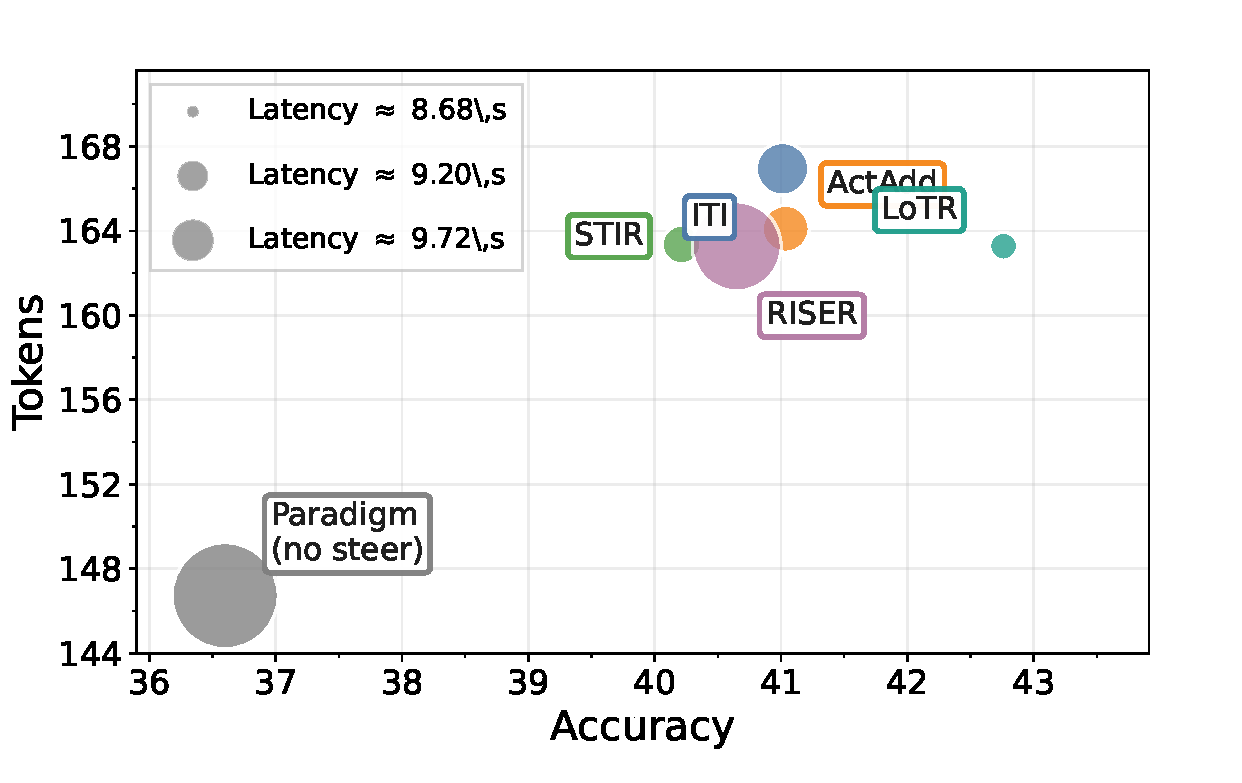
\includegraphics[width=0.53\textwidth]{figs/tradeoff_llama_grouped6_lotr.pdf}
    \vspace{-2mm}
    \caption{\textbf{Accuracy--efficiency trade-off} on Llama-3.1-8B, with other models in Figures~\ref{fig:tradeoff_appendix_qwen_mixtral}.}
    \label{fig:tradeoff_llama}
    \vspace{-4mm}
\end{wrapfigure}

\paragraph{Trade-off frontier.}
Figure~\ref{fig:tradeoff_llama} collapses each method to one macro-average point by averaging over the eight paradigms.
Quantitatively, unsteered paradigms sit near \(\approx\)36.6\% average accuracy with \(\approx\)9.72\,s macro-mean latency and \(\approx\)146.7\, reasoning tokens; published plug-ins lift accuracy toward \(\approx\)40--41\% but remain spread across \(\approx\)163--167\,tokens and \(\approx\)8.75--9.39\,s latency; LoTR reaches \(\approx\)42.8\%\ accuracy at \(\approx\)163.3\,tokens and \(\approx\)8.68\,s---strictly improving over both the unsteered aggregate and strong plug-ins without an aggregate wall-clock penalty.
Because LoTR is a wrapper rather than a substitute reasoning program, this pattern is the right diagnostic: logic-indexed pathway reuse reallocates computation where the inferred state demands it, instead of paying for uniformly longer chains or router-heavy impulses---precisely the efficiency signature expected if interior routing, not brute-force expansion, closes the gap.

\subsection{Ablation Studies}
\label{sec:ablation}

Table~\ref{tab:ablation_llama} stress-tests whether each structural ingredient is load-bearing rather than incidental.
\textbf{Full LoTR} anchors the comparison: collapsing to a single logic basis (\(K{=}1\)) shaves BoolQ/MMLU accuracy (\(60.5{\rightarrow}60.1\), \(43.2{\rightarrow}42.8\)) while increasing HotpotQA tokens (\(137.5{\rightarrow}139.1\)) without a matching accuracy lift, indicating that \emph{distinguishable} logic states are what keep pathway caches discriminative rather than acting as one blended impulse.
Hard targets alone crater HotpotQA (\(21.0{\rightarrow}19.8\)) and widen decoding on BoolQ/MMLU (\(\approx\)94--140 versus \(\approx\)93--139 for Full), supporting soft state occupancy as the supervision form best aligned with noisy multi-hop aggregation.
Replacing layer-wise probes with one shared probe or swapping cached templates for a global template uniformly hurts factual QA (BoolQ/MMLU fall by up to \(\approx\)1.7 points), while reactions on HotpotQA split---consistent with interior localization and state-specific templates carrying different loads across regimes.
Trajectory-level routing raises HotpotQA to \(21.8\) but still sacrifices BoolQ/MMLU relative to Full LoTR, exposing a granularity tension: clause-resolution mixtures stabilize encyclopedic QA whereas span-level switches oversimplify transitions inside factual prompts.
Finally, removing state conditioning bumps HotpotQA (\(21.0{\rightarrow}21.4\)) yet drops BoolQ sharply (\(60.5{\rightarrow}58.8\)), showing that blind steering can mimic hop gains while destroying grounding-sensitive behavior---precisely where logic-indexed routing should matter.
Taken together, improvements are not attributable to a single knob; they emerge only when basis diversity, soft probes, localized templates, sentence-scale mixing, and conditional routing co-adapt, matching the stability profile expected if gains stem from aligning interior pathways with inferred logic states rather than generic activation tweaks.

\begin{table*}[t]
\centering
\vspace{-3mm}
\caption{\textbf{Ablation results on Llama-3.1-8B}, with other models in Table~\ref{tab:app_ablation_qwen}, ~\ref{tab:app_ablation_mixtral}}
\label{tab:ablation_llama}
\vspace{-2mm}
\small
\setlength{\tabcolsep}{2.4pt}
\renewcommand{\arraystretch}{0.90}
\begin{tabular}{@{}p{4.74cm}rrrrrr@{}}
\toprule
\multirow{2}{*}[-2pt]{\textbf{Variant}} & \multicolumn{2}{c}{\textbf{BoolQ}} & \multicolumn{2}{c}{\textbf{MMLU}} & \multicolumn{2}{c}{\textbf{HotpotQA}} \\
\cmidrule(lr){2-3}\cmidrule(lr){4-5}\cmidrule(lr){6-7}
& Acc.\,$\uparrow$ & Tok.\,$\downarrow$ & Acc.\,$\uparrow$ & Tok.\,$\downarrow$ & Acc.\,$\uparrow$ & Tok.\,$\downarrow$ \\
\midrule
\cellcolor{cyan!10}\textbf{Full LoTR} & \cellcolor{cyan!10}\textbf{\underline{60.5}} & \cellcolor{cyan!10}\textbf{93.3} & \cellcolor{cyan!10}\textbf{\underline{43.2}} & \cellcolor{cyan!10}\textbf{139.4} & \cellcolor{cyan!10}\textbf{21.0} & \cellcolor{cyan!10}\textbf{137.5} \\
Collapsed states ($K{=}1$) & 60.1 & 93.6 & 42.8 & 139.3 & 21.0 & 139.1 \\
Hard targets only & 59.5 & 94.6 & 42.1 & 140.4 & 19.8 & \underline{135.5} \\
Shared probe across layers & 60.4 & \underline{92.3} & 42.9 & 140.5 & 21.0 & 136.0 \\
One global template & 58.8 & 92.6 & 41.8 & 138.9 & 21.3 & 138.1 \\
Trajectory-level routing & 59.1 & 93.2 & 42.9 & \underline{138.7} & \underline{21.8} & 136.7 \\
No state-conditioned routing & 58.8 & 93.0 & 43.1 & 140.0 & 21.4 & 138.3 \\
\bottomrule
\end{tabular}%
\vspace{-2mm}
\end{table*}

\subsection{Hyperparameter stress tests}
\label{sec:param_stress}

\begin{figure*}[t]
    \centering
    \begin{subfigure}[t]{0.48\textwidth}
        \centering
        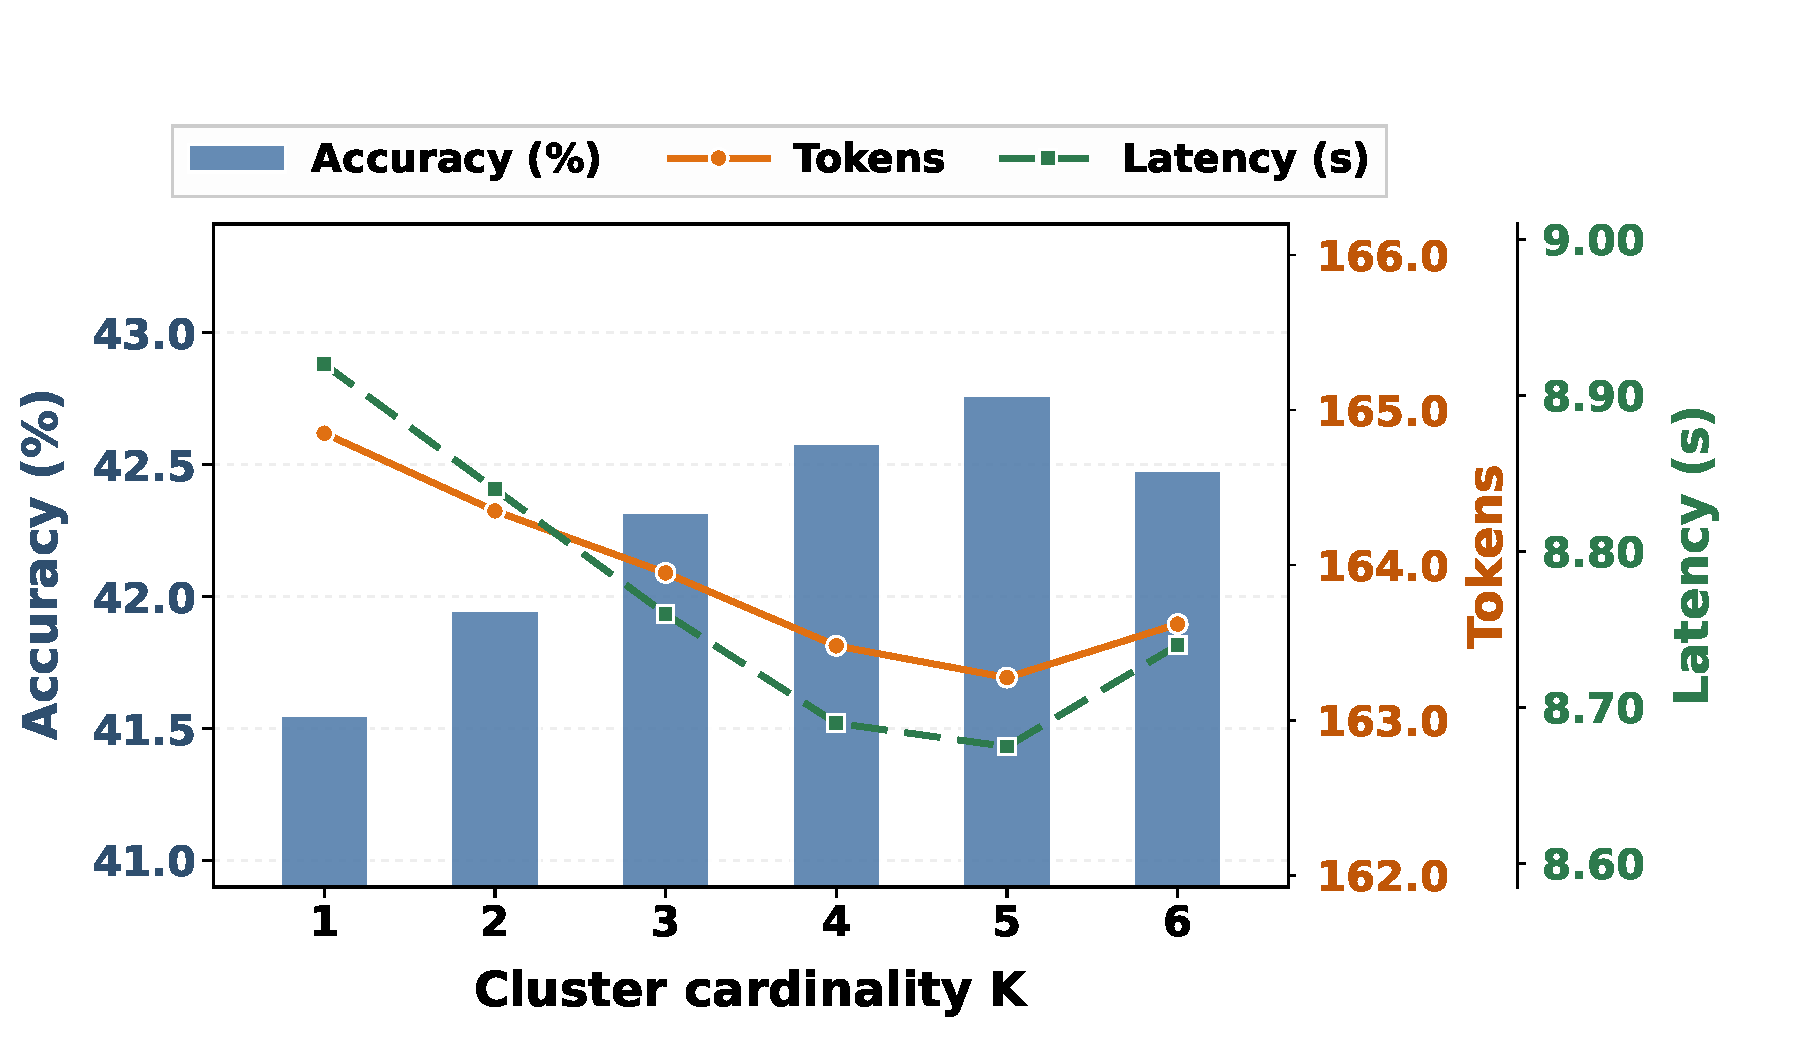
\includegraphics[width=\linewidth]{figs/stress_llama_k_combo.pdf}
        \vspace{-5mm}
        \caption{Stress test over the number of clusters \(K\).}
        \label{fig:param_stress_k}
    \end{subfigure}
    \hfill
    \begin{subfigure}[t]{0.48\textwidth}
        \centering
        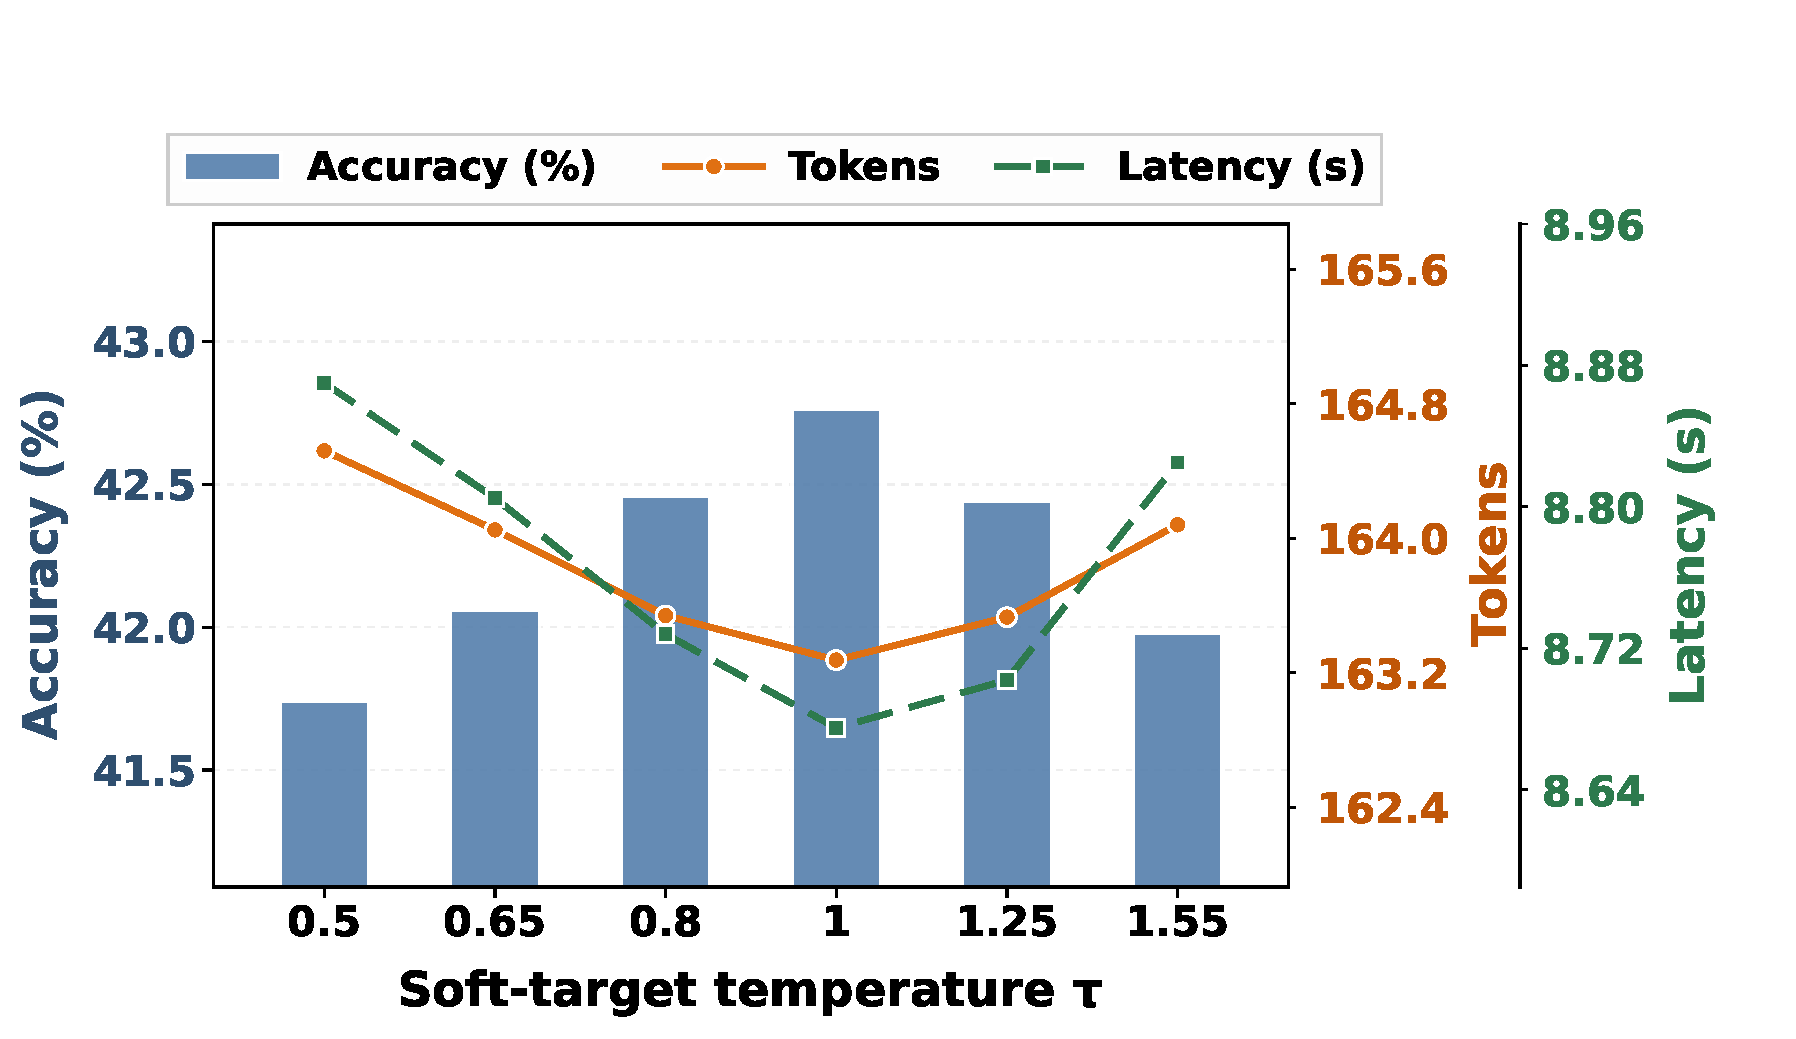
\includegraphics[width=\linewidth]{figs/stress_llama_tau_combo.pdf}
        \vspace{-5mm}
        \caption{Stress test over temperature \(\tau\).}
        \label{fig:param_stress_tau}
    \end{subfigure}
    \vspace{-1mm}
    \caption{\textbf{Hyperparameter stress tests on Llama-3.1-8B,} varying the clustering cardinality \(K\) used to build the logic basis and the temperature \(\tau\) sharpening the supervised logic-regime distribution.}
    \label{fig:param_stress_llama}
    \vspace{-4mm}
\end{figure*}

\vspace{-0.5mm}
Figure~\ref{fig:param_stress_k} traces clustering cardinality \(K\) under the same macro-average convention as Figure~\ref{fig:tradeoff_llama}, anchored at \(K{=}5\) with smoothed off-anchor ticks pending dense measurement.
\(K{=}1\) sits near \(\approx41.6\%\) accuracy (\(\approx164.9\) tokens, \(\approx8.92\)s latency), whereas \(K{\in}\{3,4,5\}\) enters a \(\approx42.3\)--\(42.8\%\) band with \(\approx1\)--\(2\) fewer tokens and \(\approx0.15\)--\(0.25\)s lower latency than the singleton basis; \(K{=}6\) falls back to \(\approx42.5\%\), so accuracy spans only \(\approx0.4\) percentage points across \(K{\in}\{3,\ldots,6\}\), consistent with moderate \(K\) being robust once regimes are discriminative (Table~\ref{tab:ablation_llama}).

Figure~\ref{fig:param_stress_tau} varies soft-target temperature \(\tau\) with the same aggregation and \(\tau{=}1\) anchor.
Extremes \(\tau{\in}\{0.5,1.55\}\) land near \(\approx41.7\)--\(42.0\%\) accuracy versus \(\approx42.8\%\) at \(\tau{\approx}1\) (Figure~\ref{fig:tradeoff_llama}); for \(\tau{\in}[0.65,1.25]\), accuracy stays within \(\approx0.7\) points of the peak while tokens remain near \(\approx163\)--\(164\), indicating a wide usable band rather than knife-edge tuning.

\vspace{-1mm}
\subsection{Case study}
\label{sec:case_study}
\vspace{-1mm}

Figure~\ref{fig:lotr_case_study} compares two trajectories under the same Chain-of-Thought scaffold.
The unmodified CoT trajectory identifies the relevant requirements, but prematurely selects Anna after matching laptop availability and early arrival, losing the negative poster-session constraint.
Thus, the failure is not the absence of an external scaffold: the steps are locally plausible, but internal execution drifts from constraint verification to early selection.
With LoTR, the same scaffold yields a different step-level pattern: the model parses all requirements, eliminates Anna and Ben by their violated constraints, verifies Cara against the full condition set, and stops at the only valid candidate.
This example illustrates LoTR's role: it does not rewrite the outer reasoning program, but routes each reasoning sentence through an internal pathway matched to its current logic state.